\documentclass[a4paper, 12pt]{article}
\usepackage{barinovlab}
\usepackage[many]{tcolorbox}
\usepackage{calc}
\begin{document}
\thispagestyle{empty}
\begin{center}
    \textit{Федеральное государственное автономное образовательное\\ учреждение высшего образования }

    \vspace{0.5ex}

        \textbf{«Московский физико-технический институт\\ (национальный исследовательский университет)»}
\end{center}

\vspace{10ex}

\begin{center}
    \vspace{13ex}

    \so{\textbf{Лабораторная работа №_._._}}

    \vspace{1ex}

    по курсу общей физики

    на тему:

    \textbf{\textit{<<>>}}

    \vspace{30ex}

    \begin{flushright}
        \noindent
        \textit{Работу выполнил:}\\  
        \textit{Баринов Леонид \\(группа Б02-827)}
    \end{flushright}
    \vfill
    Долгопрудный \\2019
\newpage
\setcounter{page}{1}
\fancyhead[R]{\nouppercase{\leftmark}}	
\end{center}

\section{Аннотация}
В работе будет рассмотрена сферическая аберрация на одной линзе и на
паре центрированных линз, будут подобраны параметры, которые минимизируют сферическую
аберрацию в обоих случаях c помощью моделирования в <<Wolfram
Mathematica>>. Из дифракционной оценки будет получено возможное оптимальное
положение экрана.

\section{Теоретические сведения}
\textit{Аберрации оптической системы} --- это ошибки или дефекты
изображения в реальной оптической системе, вызываемые отклонением
лучей от того направления, по которому они должны были бы идти в
идеальной оптической системе.

\textit{Сферическая аберрация} \ffig{fig:1} возникает из-за несовпадения фокусов
для лучей света, проходящих на разных расстояниях от оптической оси и
приводит к нарушению гомоцентричности пучков лучей от точечного
источника, без нарушения симметрии строения этих пучков.

%\begin{figure}[H]
%    \def\svgscale{0.5}
%    \input{images/2.pdf_tex}
%    \caption{}
%    \label{}
%\end{figure}

\begin{figure}[H]
    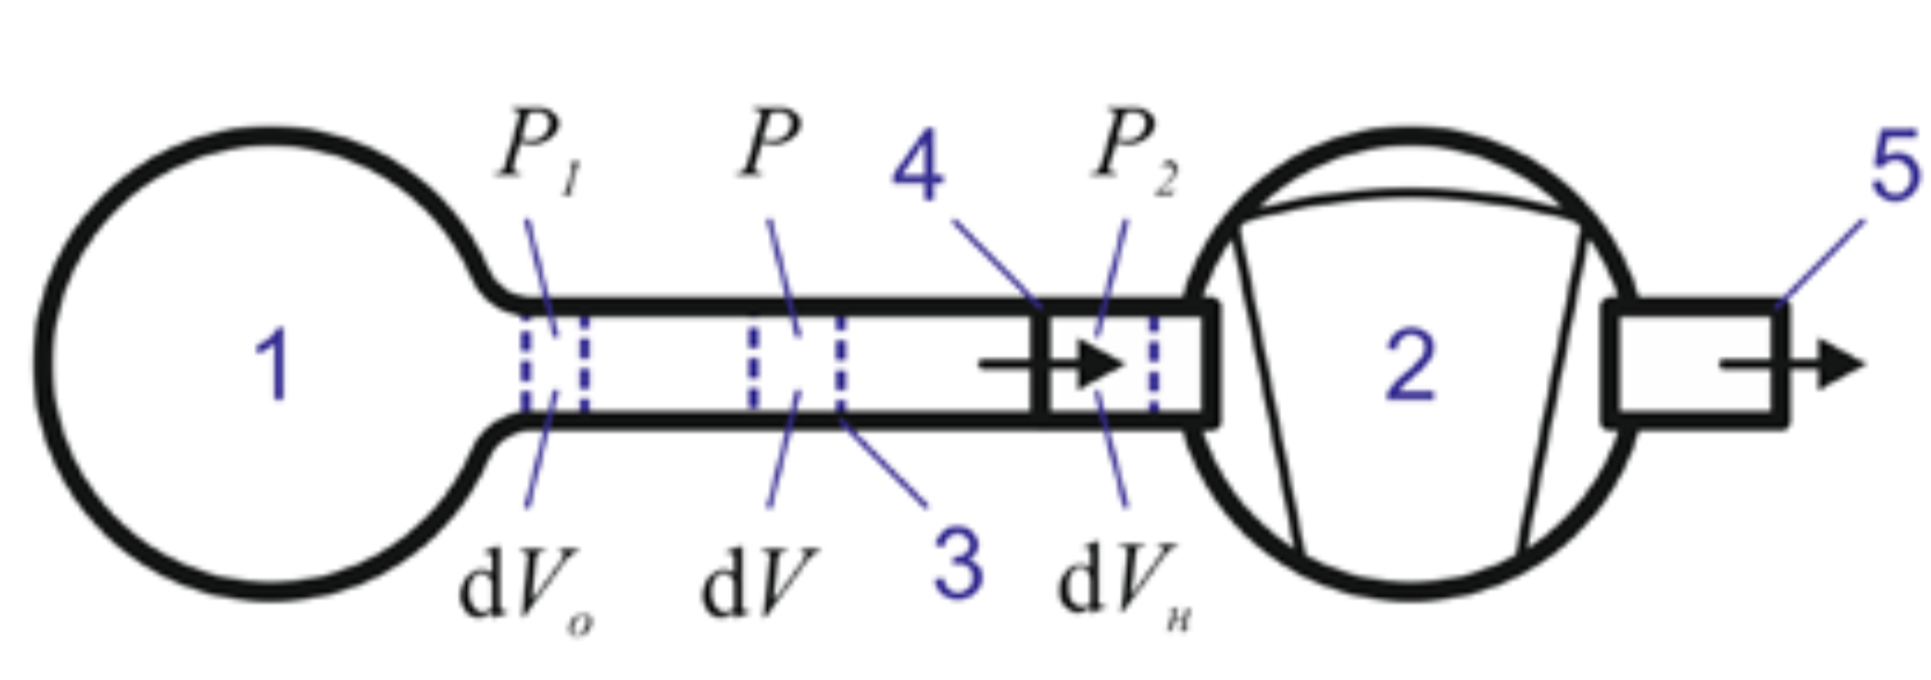
\includegraphics[width=0.6\linewidth]{1} 
    \caption{Сферическая аберрация}
    \label{fig:1}
\end{figure}

Фокусное расстояние линзы определяется через радиусы сферических
поверхностей, ее ограничивающих:
\begin{equation}
    \frac{1}{F} = (n-1) \left( \frac{1}{R_1}+ \frac{1}{R_2} \right) 
    \label{eq:1}
\end{equation}

Для исследования аберраций рассмотрим преломление луча на сферической
поверхности.
\begin{figure}[H]
    \def\svgscale{1.1}
    \input{images/2.pdf_tex}
    \caption{Преломление луча на сферической поверхности}
    \label{fig:2}
\end{figure}

Исходя из рисунка запишем соотношения:
\begin{equation}
    \begin{aligned}
        i_1 &= \phi_1+\alpha = \phi_1 + \arcsin \frac{y_1}{R}\\
        i_2 &= \phi_2+\alpha = \phi_2 + \arcsin \frac{y_1}{R}
    \end{aligned}
    \label{eq:2}
\end{equation}

Воспользуемся законом Снеллиуса
\begin{equation}
    n_1 \sin i_1 = n_2 \sin i_2
    \label{eq:3}
\end{equation}
и выразим $\phi_2$ из \eqref{eq:2} через $\phi_1$, $n_1$, $n_2$, $R$ и
$y_1$.
\begin{equation}
    \phi_2 = \arcsin \left( \frac{n_1}{n_2} \sin \left( \phi_1 +
    \arcsin \frac{y_1}{R} \right) \right) - \arcsin \frac{y_1}{R}
    \label{eq:4}
\end{equation}

Рассуждения для следующего преломления аналогичны, меняется только
знак $R$ и $\phi$. Знаки перед $R$ и $\phi$ ставятся согласно
\fig{fig:2a}.
\begin{figure}[H]
    \def\svgscale{0.8}
    \input{images/2a.pdf_tex}
    \caption{Расстановка знаков перед $R$ и $\phi$}
    \label{fig:2a}
\end{figure}


Для определения продольной $X$ и поперечной $Y$ компонент сферической аберрации поместим
объект в двойной фокус собирающей линзы. Для остальных положений
объекта рассуждения будут аналогичными. Из формулы тонкой линзы
следует, что изображение также
будет в $2F$, однако это выполняется только в параксиальном
приближении, это хорошо видно на \fig{fig:3}.
\begin{figure}[H]
    \def\svgscale{1.3}
    \input{images/3.pdf_tex}
    \caption{Продольная $X$ и поперечная $Y$ компоненты сферической аберрации}
    \label{fig:3}
\end{figure}

Значения $X$ и $Y$ находим по углу $\phi_\text{out}$ между крайним
преломленным лучом и главной оптической осью. $H$ --- высота
линзы.
\begin{equation}
    \begin{aligned}
        X &= 2F-H/2\ctg \phi_\text{out}\\
        Y &= 2F\tg \phi_\text{out} - H/2 
    \end{aligned}
    \label{eq:5}
\end{equation}

Поставим задачу наилучшего положения экрана $\text{Э}$ между
положениями $\text{Э}_1$ и $\text{Э}_2$. Для этого разобьем половину
линзы на $N$ частей (на \fig{fig:3} $N=4$). Положение $\text{Э}_1$
получается из пересечения крайними лучами главной оптической оси.
Положение $\text{Э}_2$ получается из пересечения лучами, которые
попадают на границу $1$ области линзы, главной
оптической оси. Параметром наилучшего положения будем считать
интенсивность и радиус кружка изображения каждой зоны $N$.

Рассчитаем интенсивность каждого кружка и его радиус. Выразим телесный
угол $\Omega_n$, под которым видна $n$ зона
\begin{equation}
    \begin{gathered}
    \Omega_n = \frac{\pi(y_n^2-y_{n-1}^2)}{(2F)^2+y_n^2}\cos
    \phi_{\text{in}} \\
    \cos \phi_\text{in} = \frac{2F}{\sqrt{(2F)^2 + y_n^2}} =
    \frac{N}{\sqrt{N^2 + \left( \frac{Hn}{4F} \right)^2}}
\end{gathered}
    \label{eq:6}
\end{equation}
$y_n$ --- расстояние от центра линзы $O$ до окончания $n$-ой зоны,
$y_{n-1}$ --- расстояние от центра линзы $O$ до окончания $n-1$-ой
зоны.

Рассчитаем какая часть энергии $\omega_n$ в единицу времени содержится
в выделенном телесном угле
$\Omega_n$:
\begin{equation}
    \omega_n = \omega_0 \frac{\Omega_n}{4\pi} = \frac{\omega_0}{4}\cdot
    \frac{y_n^2-y_{n-1}^2}{(2F)^2+y_n^2}\cos \phi_\text{in}
    \label{eq:7}
\end{equation}
$\omega_0$ --- суммарная энергия, выходящая из источника в единицу
времени.

Выразим интенсивность $I_n$:
\begin{equation}
    I_n = \frac{\omega_n}{\pi(Y_n^2-Y_{n-1}^2)} =
    \frac{\omega_0}{4\pi} \frac{y_n^2-y_{n-1}^2}{(2F)^2+y_n^2}\cdot
    \frac{\cos \phi_\text{in}}{Y_n^2-Y_{n-1}^2}
    \label{eq:8}
\end{equation}
$Y_n$ --- радиус $n$-ой зоны, получаемой на экране в положении
$\text{Э}_2$, $Y_{n-1}$ ---
радиус $n-1$-ой зоны, получаемой на экране в положении $\text{Э}_2$.

Радиус $y_n$ можно выразить через $H$ и $N$:
\[
    y_n = \frac{H}{2 N} n
\]
Перепишем выражение $y_n^2-y_{n-1}^2$:
\[
    y_n^2-y_{n-1}^2 = \left( \frac{H}{2 N} \right)^2 (n^2-(n-1)^2) =
    \left( \frac{H}{2 N} \right)^2 (2n+1)
\]

Перепишем \eqref{eq:8}:
\begin{equation}
    I_n = \frac{\omega_0}{16\pi F^2} \left( \frac{H}{2 N} \right)^2
    \frac{\cos\phi_\text{\text{in}}}{1+\left( \frac{D}{4 N F}n \right)^2} \cdot
    \frac{2n+1}{Y_n^2-Y_{n-1}^2}
    \label{eq:9} 
\end{equation}

Константу в формуле \eqref{eq:9} обозначим за $I_0$:
\[
    I_0 = \frac{\omega_0}{16\pi F^2}\left( \frac{H}{2} \right)^2
\]

В итоге формула \eqref{eq:9} принимает вид:
\begin{equation}
    \tcboxmath[colback=white, boxrule=1pt]{I_n = I_0
        \frac{N}{\left[ N^2+\left( \frac{Dn}{4F}
        \right)^2\right]^{3/2}} \cdot
    \frac{2n+1}{Y_n^2-Y_{n-1}^2}}
    \label{eq:10}
\end{equation}

При этом $Y_n$ соответствует величине поперечной компоненты
сферической аберрации для $n$-ой зоны, которую можно вычислить по
формуле \eqref{eq:5}, заменяя в этой формуле угол $\phi_\text{out}$ на
угол $\phi_2$ в формуле \eqref{eq:4}. 

Отметим, что формула \eqref{eq:10} получена для положения экрана
$\text{Э}_2$. Получить зависимость интенсивности для произвольного
положения экрана между $\text{Э}_1$ и $\text{Э}_2$ достаточно
затруднительно из-за нетривиального пересечения зон (это хорошо видно
при положении экрана $\text{Э}_1$ на \fig{fig:3}), однако радиус пятна
получить возможно. Для этого необходимо выбрать зону, имеющую
максимальный радиус при данном положении экрана. Например, для
$\text{Э}_1$ на \fig{fig:3} это будет вторая зона.

Для определения наилучшего положения экрана воспользуемся
дифракционными соображениями. То есть потребуем, чтобы размер пятна
был определен исходя
из дифракционной оценки:
\begin{equation}
    D = \frac{\lambda}{H}\cdot 2F
    \label{eq:11}
\end{equation}
При этом под радиусом пятна будем понимать именно радиус того пятна, в котором
интенсивность наибольшая, т.е. не будем учитывать лучи, которые уже
пересеклись на главной оптической оси, а затем попали на экран. 

Будем помещать экран в положения, где лучи от какой-нибудь зоны
пересекли главную оптическую ось, таких положений будет $N$. Из
прямоугольного треугольника, образованного главной оптической осью,
осью линзы и лучом от $k$ зоны легко выразить расстояние от положения
экрана $\text{Э}_2$:
\begin{equation}
    X_k = 2F-H/2 \ctg{\phi_k}
    \label{eq:12}
\end{equation}
где $\phi_k$ --- угол между главной оптической осью и лучом от
$k$ зоны. 

Для оценки радиуса пятна будем использовать все зоны, которые меньше
$k$. Возьмем зону $l$, $l<k$, и оценим радиус пятна, создаваемый этой
зоной:
\begin{equation}
    z_l^k = (X_k-X_{l})\tg \phi_{l}
    \label{eq:13}
\end{equation}

Получив набор значений $z_l^k$, нам необходимо выбрать максимум по всем
значениям $l$. Это и будет являться радиусом пятна $z_k$ в положении экрана
$X_k$.

Затем остается лишь подобрать такое значение $z_k$, которое будет
максимально близко к нашей дифракционной оценке $D$. 

\section{Моделирование в Wolfram Mathematica}
В первой визуализации ставится задача минимизации
поперечной компоненты сферической аберрации при заданном фокусном
расстоянии линзы $F_0$ и ее высоты $H$. Строится график зависимости
поперечной компоненты
сферической аберрации $X$ от радиуса кривизны одной из поверхностей. Так
как фокусное расстояние линзы задано, то кривизна второй поверхности
определяется по формуле \eqref{eq:1} \ffig{fig:4}.

Из графиков видно, что при увеличении отношения $F_0/H$ минимальное
значение поперечной компоненты сферической аберрации уменьшается, при
уменьшении $F_0/H$ --- увеличивается. При стремлении $n$ к $\infty$
$X$ стремится к $0$.



\begin{figure}[H]
    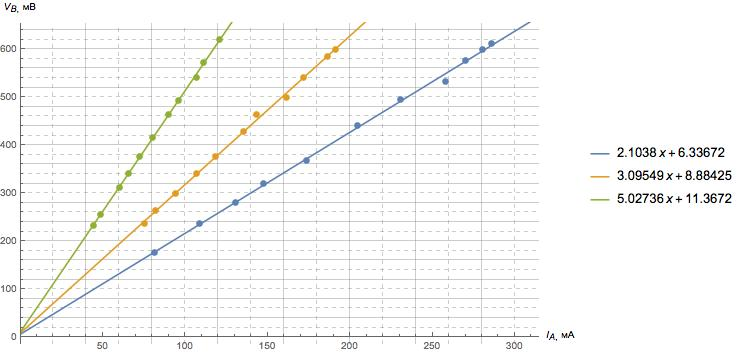
\includegraphics[width=0.8\linewidth]{12} 
    \caption{Зависимость продольной компоненты сферической аберрации
    $X$ от радиуса кривизны одной из поверхностей линзы $1/R_1$ при
различных значениях фокусного расстояния $F_0$, высоты линзы $H$ и
показателя преломления материала линзы $n$}
\label{fig:4}
\end{figure}

Целью второй визуализации ставится проверка правила <<4П>> --- <<плоской
поверхностью к плоской волне плохо>> для плоско-выпуклой линзы. Для этого нужно взять $\phi_2 = 0$
\ffig{fig:2} и заменить $2F$ на $F$ в формуле
\eqref{eq:5}. В \textsl{таблице \ref{table:1}} значения для продольной и
поперечной аберрации при $F_0=40$, $H=10$ и $n=1,5$. В первом случае
плоская волна падает на плоскую поверхность, во втором случае --- на
сферическую поверхность.

\renewcommand{\arraystretch}{1.2}
\begin{table}[H]
\centering
\begin{tabular}{|c|c|}
    \hline 
    $X_1 = 2,259$ & $X_2 = 1,164$ \\ \hline 
    $Y_1 = 0,299$ & $Y_2 = 0,150$ \\ \hline 
\end{tabular}
\caption{Значения для продольной и
поперечной\\ аберрации при $F_0=40$, $H=10$ и $n=1,5$}
\label{table:1}
\end{table}

Хорошо видно, что данное правило позволяет значительно уменьшить
сферическую аберрацию.

В следующей демонстрации рассматривается пара линз одинаковой высоты
$H$, плотно прижатых
друг к другу (получившиеся линза должна быть собирающей). Наша задача получить оптическую
систему с минимальной продольной компонентой сферической аберрации с заданным фокусным
расстоянием $F_0$, варьируя радиусы линз. Показатели преломления $n_1$
и $n_2$ не подбирались, так как $X$ минимальна при наибольших
возможных значениях $n_1$ и $n_2$.

В случае двух линз можно добиться того, что любой из $N$ лучей
попадет точно в место, предсказанное геометрической оптикой. Для
простоты рассмотрим лучи, идущие параллельно главной оптический оси,
они должны пересечься в фокусе. Сначала подберем параметры так, что
крайний луч будет попадать в фокус \ffig{fig:5}. При этом под
продольной компонентой сферической аберрации $X$ для $n$-луча будем понимать
расстояние от точки пересечения $n$-луча главной оптической осью и
фокусным расстоянием $F$. На \fig{fig:5} все лучи пересекают главную
оптическую ось до $F$.
\begin{figure}[H]
    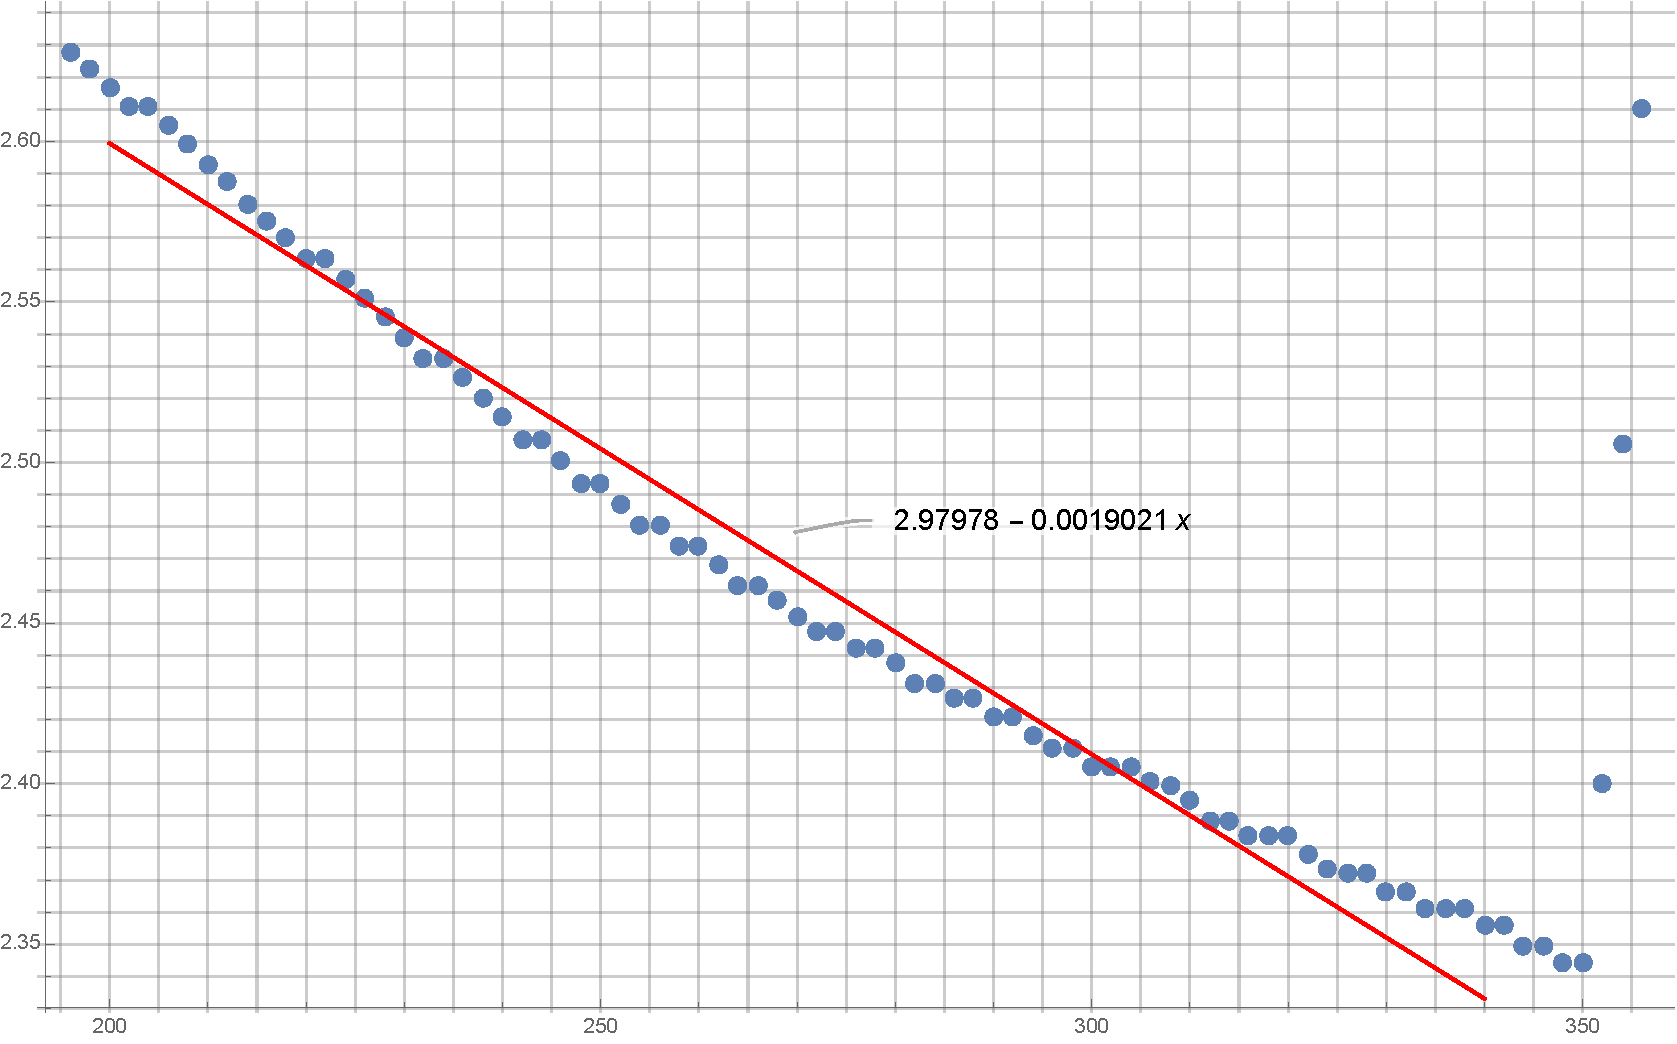
\includegraphics[width=0.7\linewidth]{13} 
    \caption{График зависимости продольной компоненты сферической
аберрации системы линз $X$ от высоты линз $H$}
\label{fig:5}
\end{figure}

При этом максимальное значение $X_{\text{max}} = 0,0262$, при этом минимальное значение
для одной линзы $X_1 = 0,761$, то есть аберрация уменьшилась более чем
в 10 раз.

Уменьшим значение $X_{\text{max}}$ c помощью переисправления
аберрации, то есть занулим аберрацию для $n$-луча, $n<N$. При этом в
первом случае будем искать минимальное значение
$X_{\text{max}}-X_{\text{min}}$, а во втором случае --- минимальное
значение $|X_{\text{max}}|$. На рисунке зеленым цветом показан первый
случай и красным второй. 

\begin{figure}[H]
    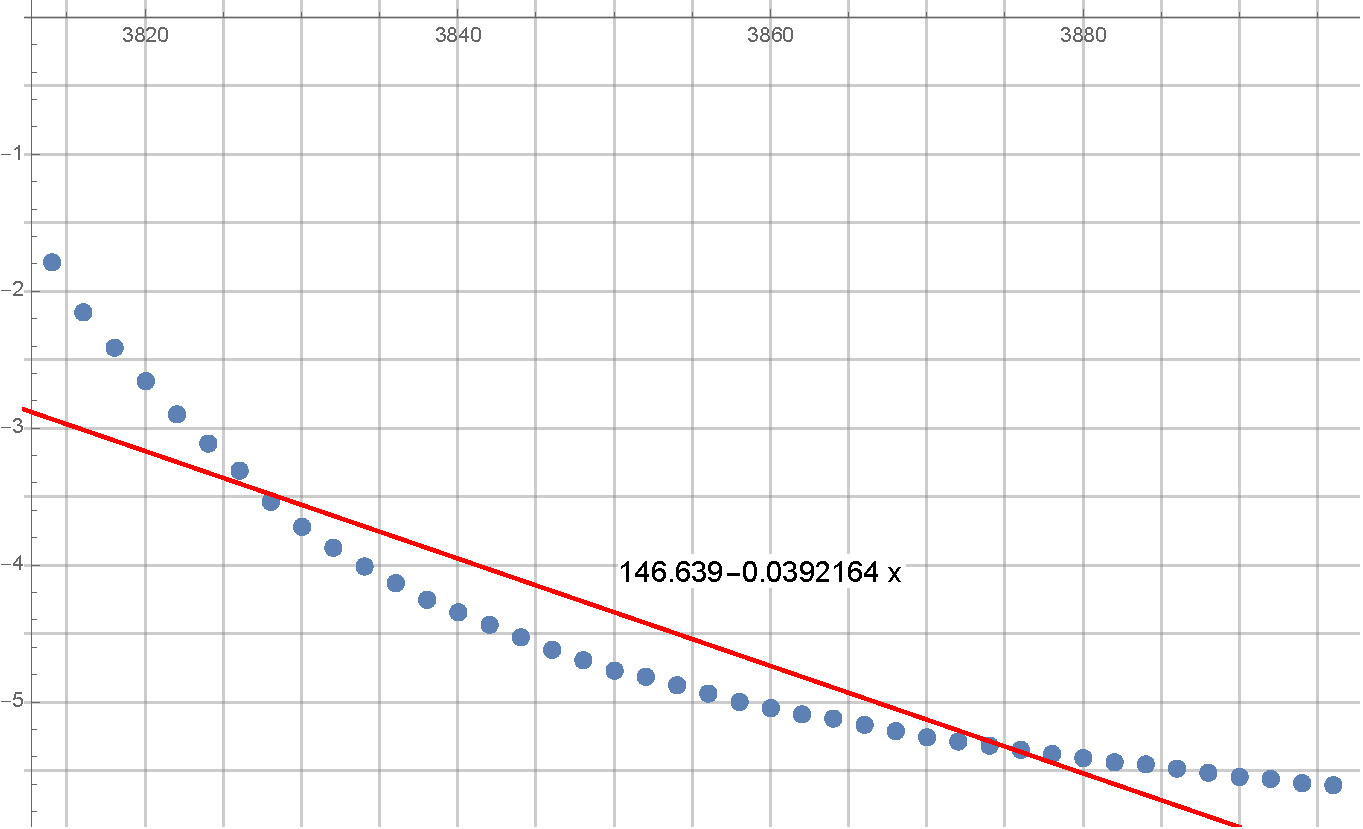
\includegraphics[width=0.8\linewidth]{14} 
    \caption{Поиск наименьшего значения
        $X_{\text{max}}-X_{\text{min}}$ (зеленая линия) и
        $|X_{\text{max}}|$ (красная линия) при различных
    значениях $H$}
\label{fig:5a}
\end{figure}

Первый случай максимально уменьшает значение продольной компоненты
сферической аберрации, делая ее равной $0,0260$. Второй же случай
показывает такую аберрацию, при который $F$ будет находится
практически по
середине между точками пересечения главной оптической оси первым и $N$
лучом.

В следующей демонстрации исследуется распределение интенсивности
внутри кружка-изображения от каждой из зон на $\fig{fig:3}$ в
положении экрана $\text{Э}_2$.
Интенсивность кружка определяется насыщенностью цвета: чем более яркий
кружок, тем больше его интенсивность. На графиках представлена
зависимость интенсивности $I$ и зависимость радиуса пятна $R$
от номера зоны $N$.


\begin{figure}[H]
    \floatsetup{heightadjust=object,valign=c}
    \begin{floatrow}

        \ffigbox{
        \caption{График зависимости интенсивности $I$ от номера зоны
        $N$}
        \label{fig:6}
    }
        {
        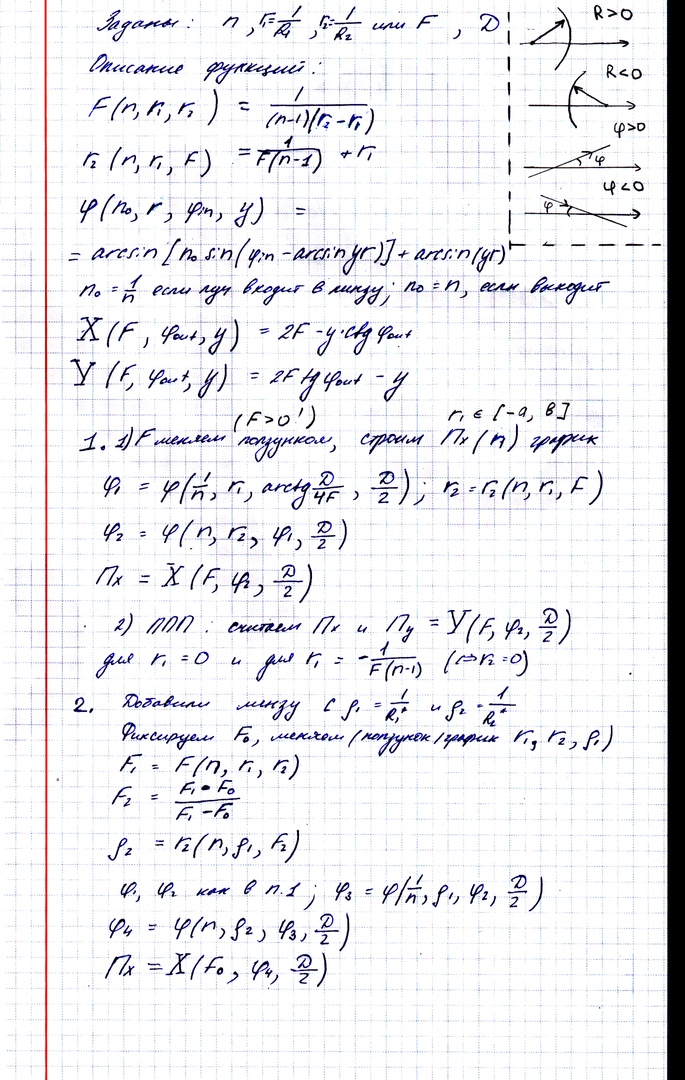
\includegraphics[width=0.8\linewidth]{6}
    }

        \ffigbox{
        \caption{График зависимости радиуса пятна $R$ от номера зоны
        $N$}
        \label{fig:7}
    }
        {
        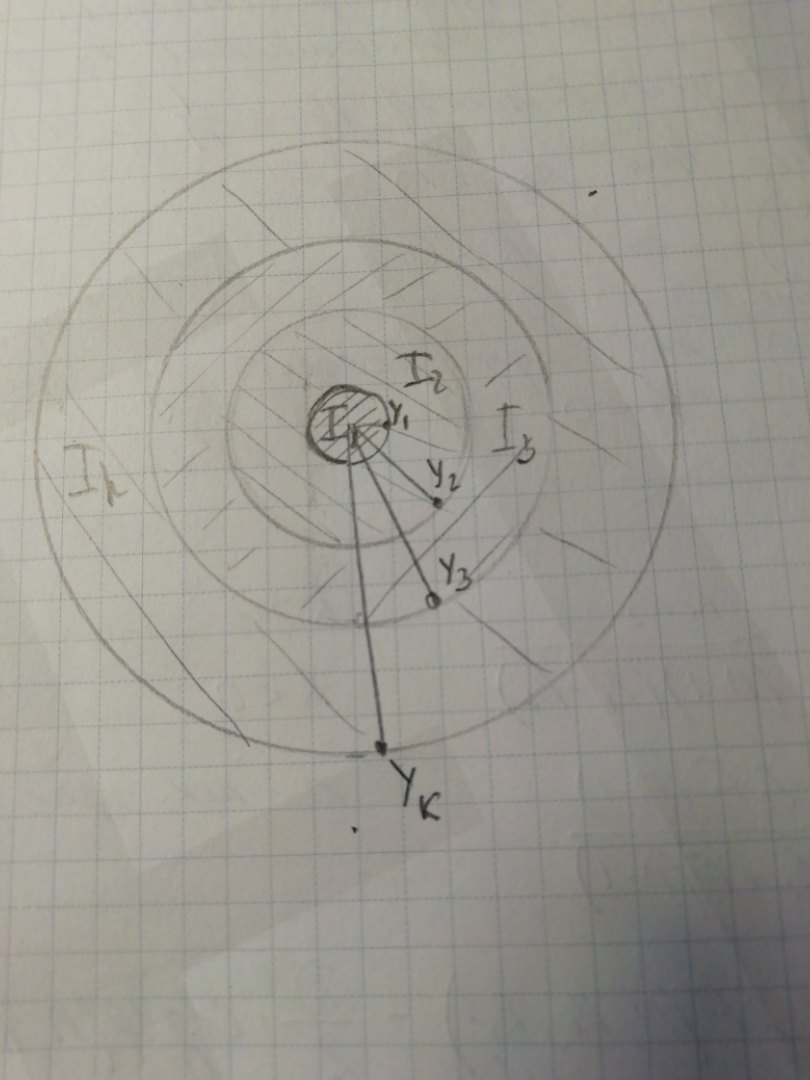
\includegraphics[width=0.8\linewidth]{7}
    }
    \end{floatrow}
\end{figure}

Так как интенсивность кружков резко падает \ffig{fig:6}, а
их радиус быстро растет \ffig{fig:7}, то в реальности мы увидим не
более 3-5 кружков, в которых интенсивность максимальна. 

\begin{figure}[H]
    \floatsetup{heightadjust=object,valign=c}
    \begin{floatrow}

        \ffigbox{
        \caption{Визуализация зависимости интенсивности $I$ и радиуса пятна $R$ от
    номера кружка $N$. На рисунке представлено 5 зон из 100 при положении экрана
$\text{Э}_2$ на \fig{fig:3}}
\label{fig:8}
    }
        {
        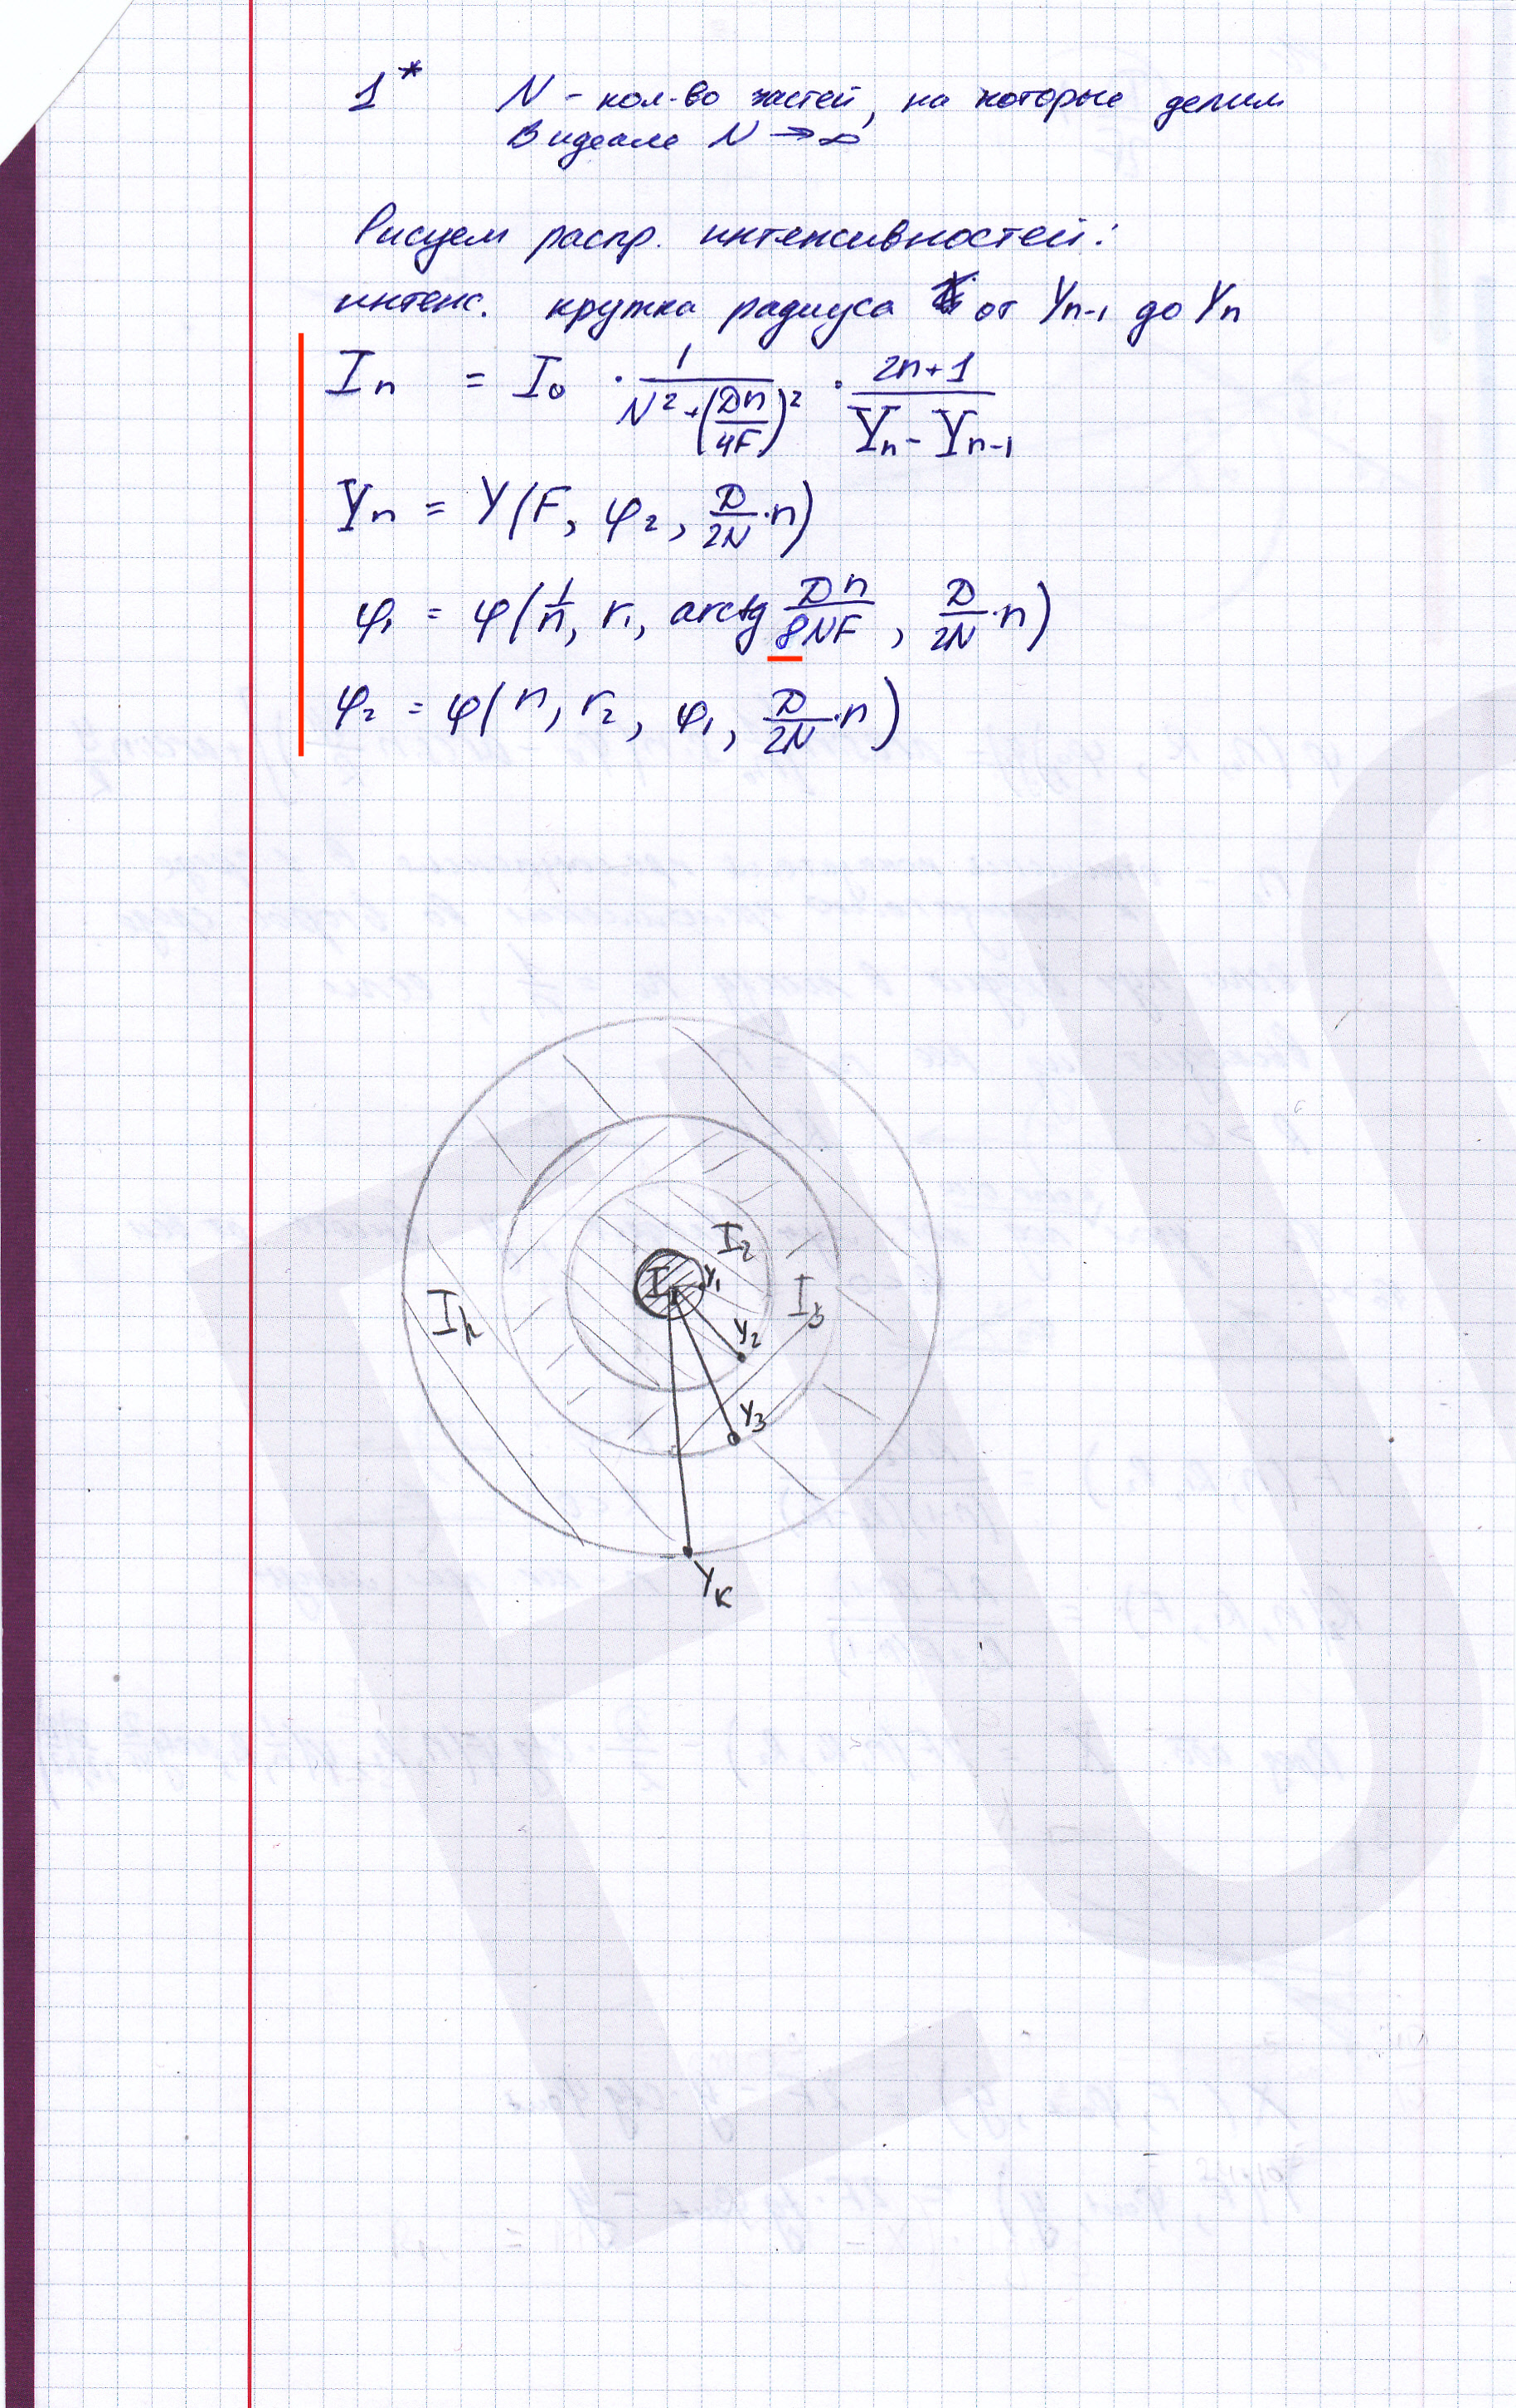
\includegraphics[width=0.8\linewidth]{8}
    }

        \ffigbox{
        \caption{Визуализация зависимости интенсивности $I$ и радиуса пятна $R$ от
    номера кружка $N$. На рисунке представлено 10 зон из 100 при положении экрана
$\text{Э}_2$ на \fig{fig:3}}
\label{fig:9}
    }
        {
        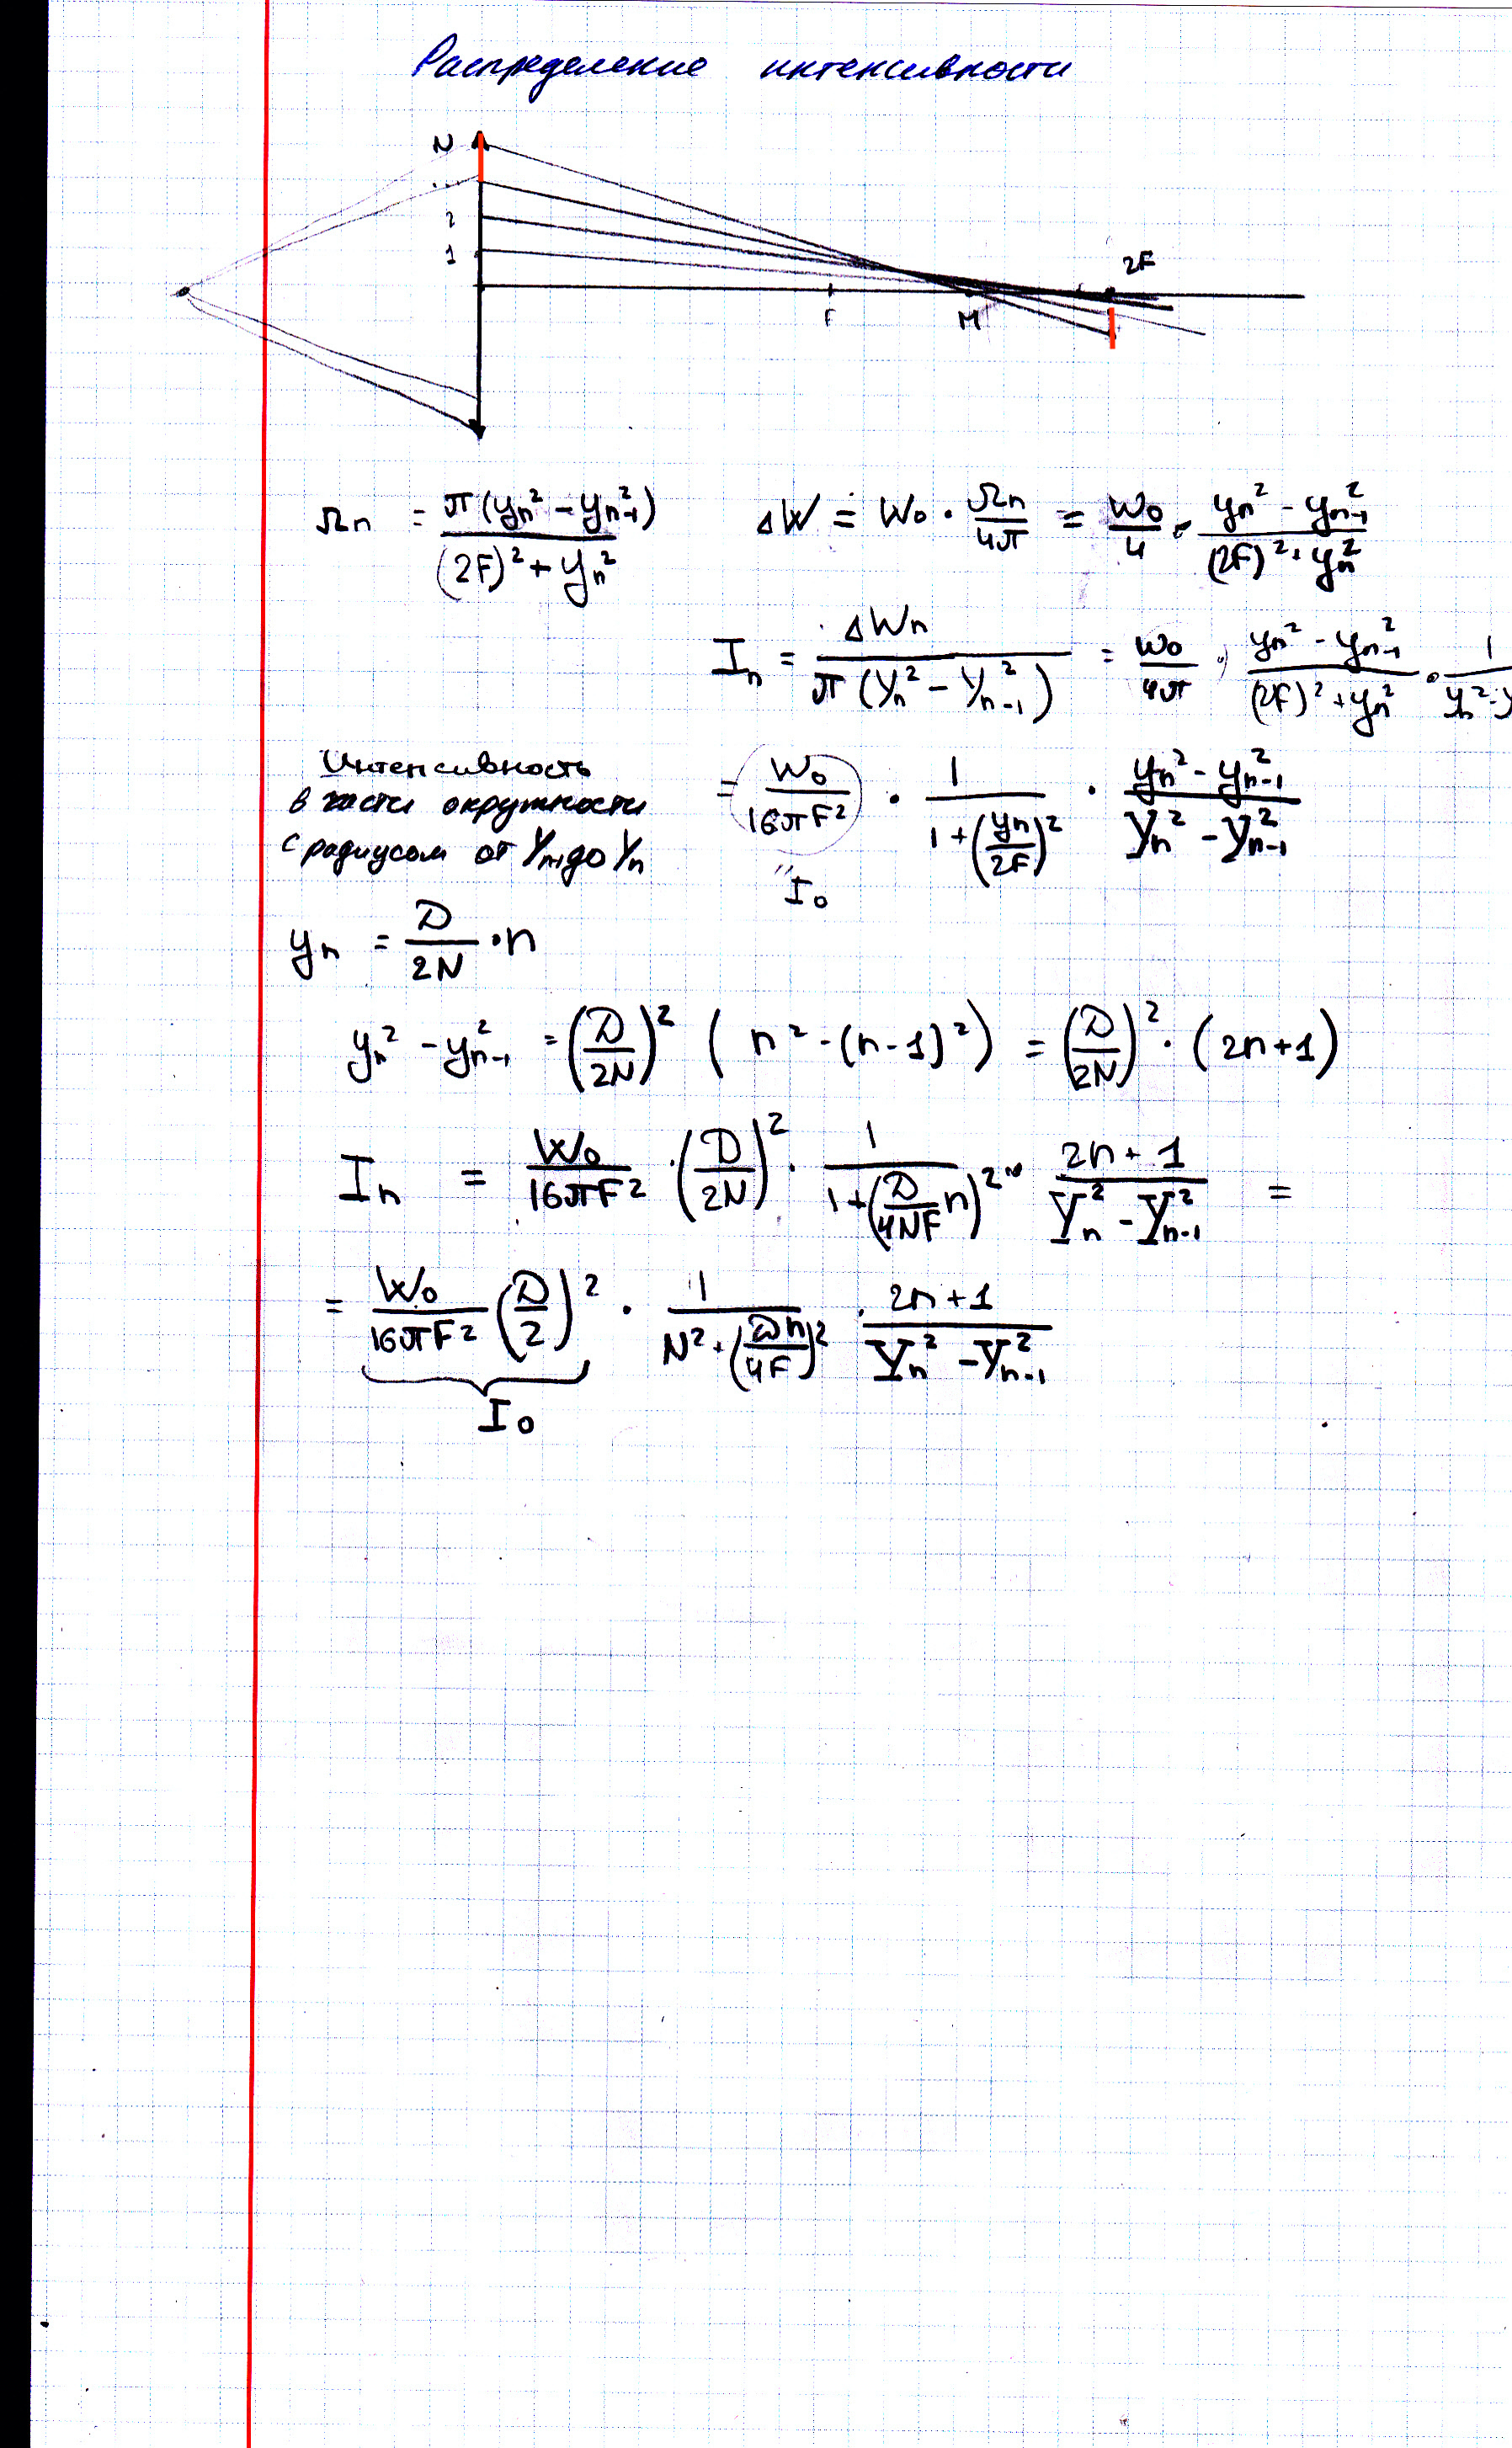
\includegraphics[width=0.8\linewidth]{9}
    }
    \end{floatrow}
\end{figure}




Вернемся к вопросу об оптимальном положении экрана. В последней
демонстрации берется значении длины волны из видимого диапазона,
исходя из этого значения по формуле \eqref{eq:11} определяется
дифракционная оценка и находится оптимальное значение $z_k$ и $X_k$ по
формулам \eqref{eq:12} и \eqref{eq:13}.

Построим график зависимости радиуса <<яркого>> пятна от $k$. При этом
$k=1$ соответствует положению экрана $\text{Э}_2$, а $k=100$ ---
положению $\text{Э}_1$. Красной точкой отметим оптимальное положение.


\begin{figure}[H]
    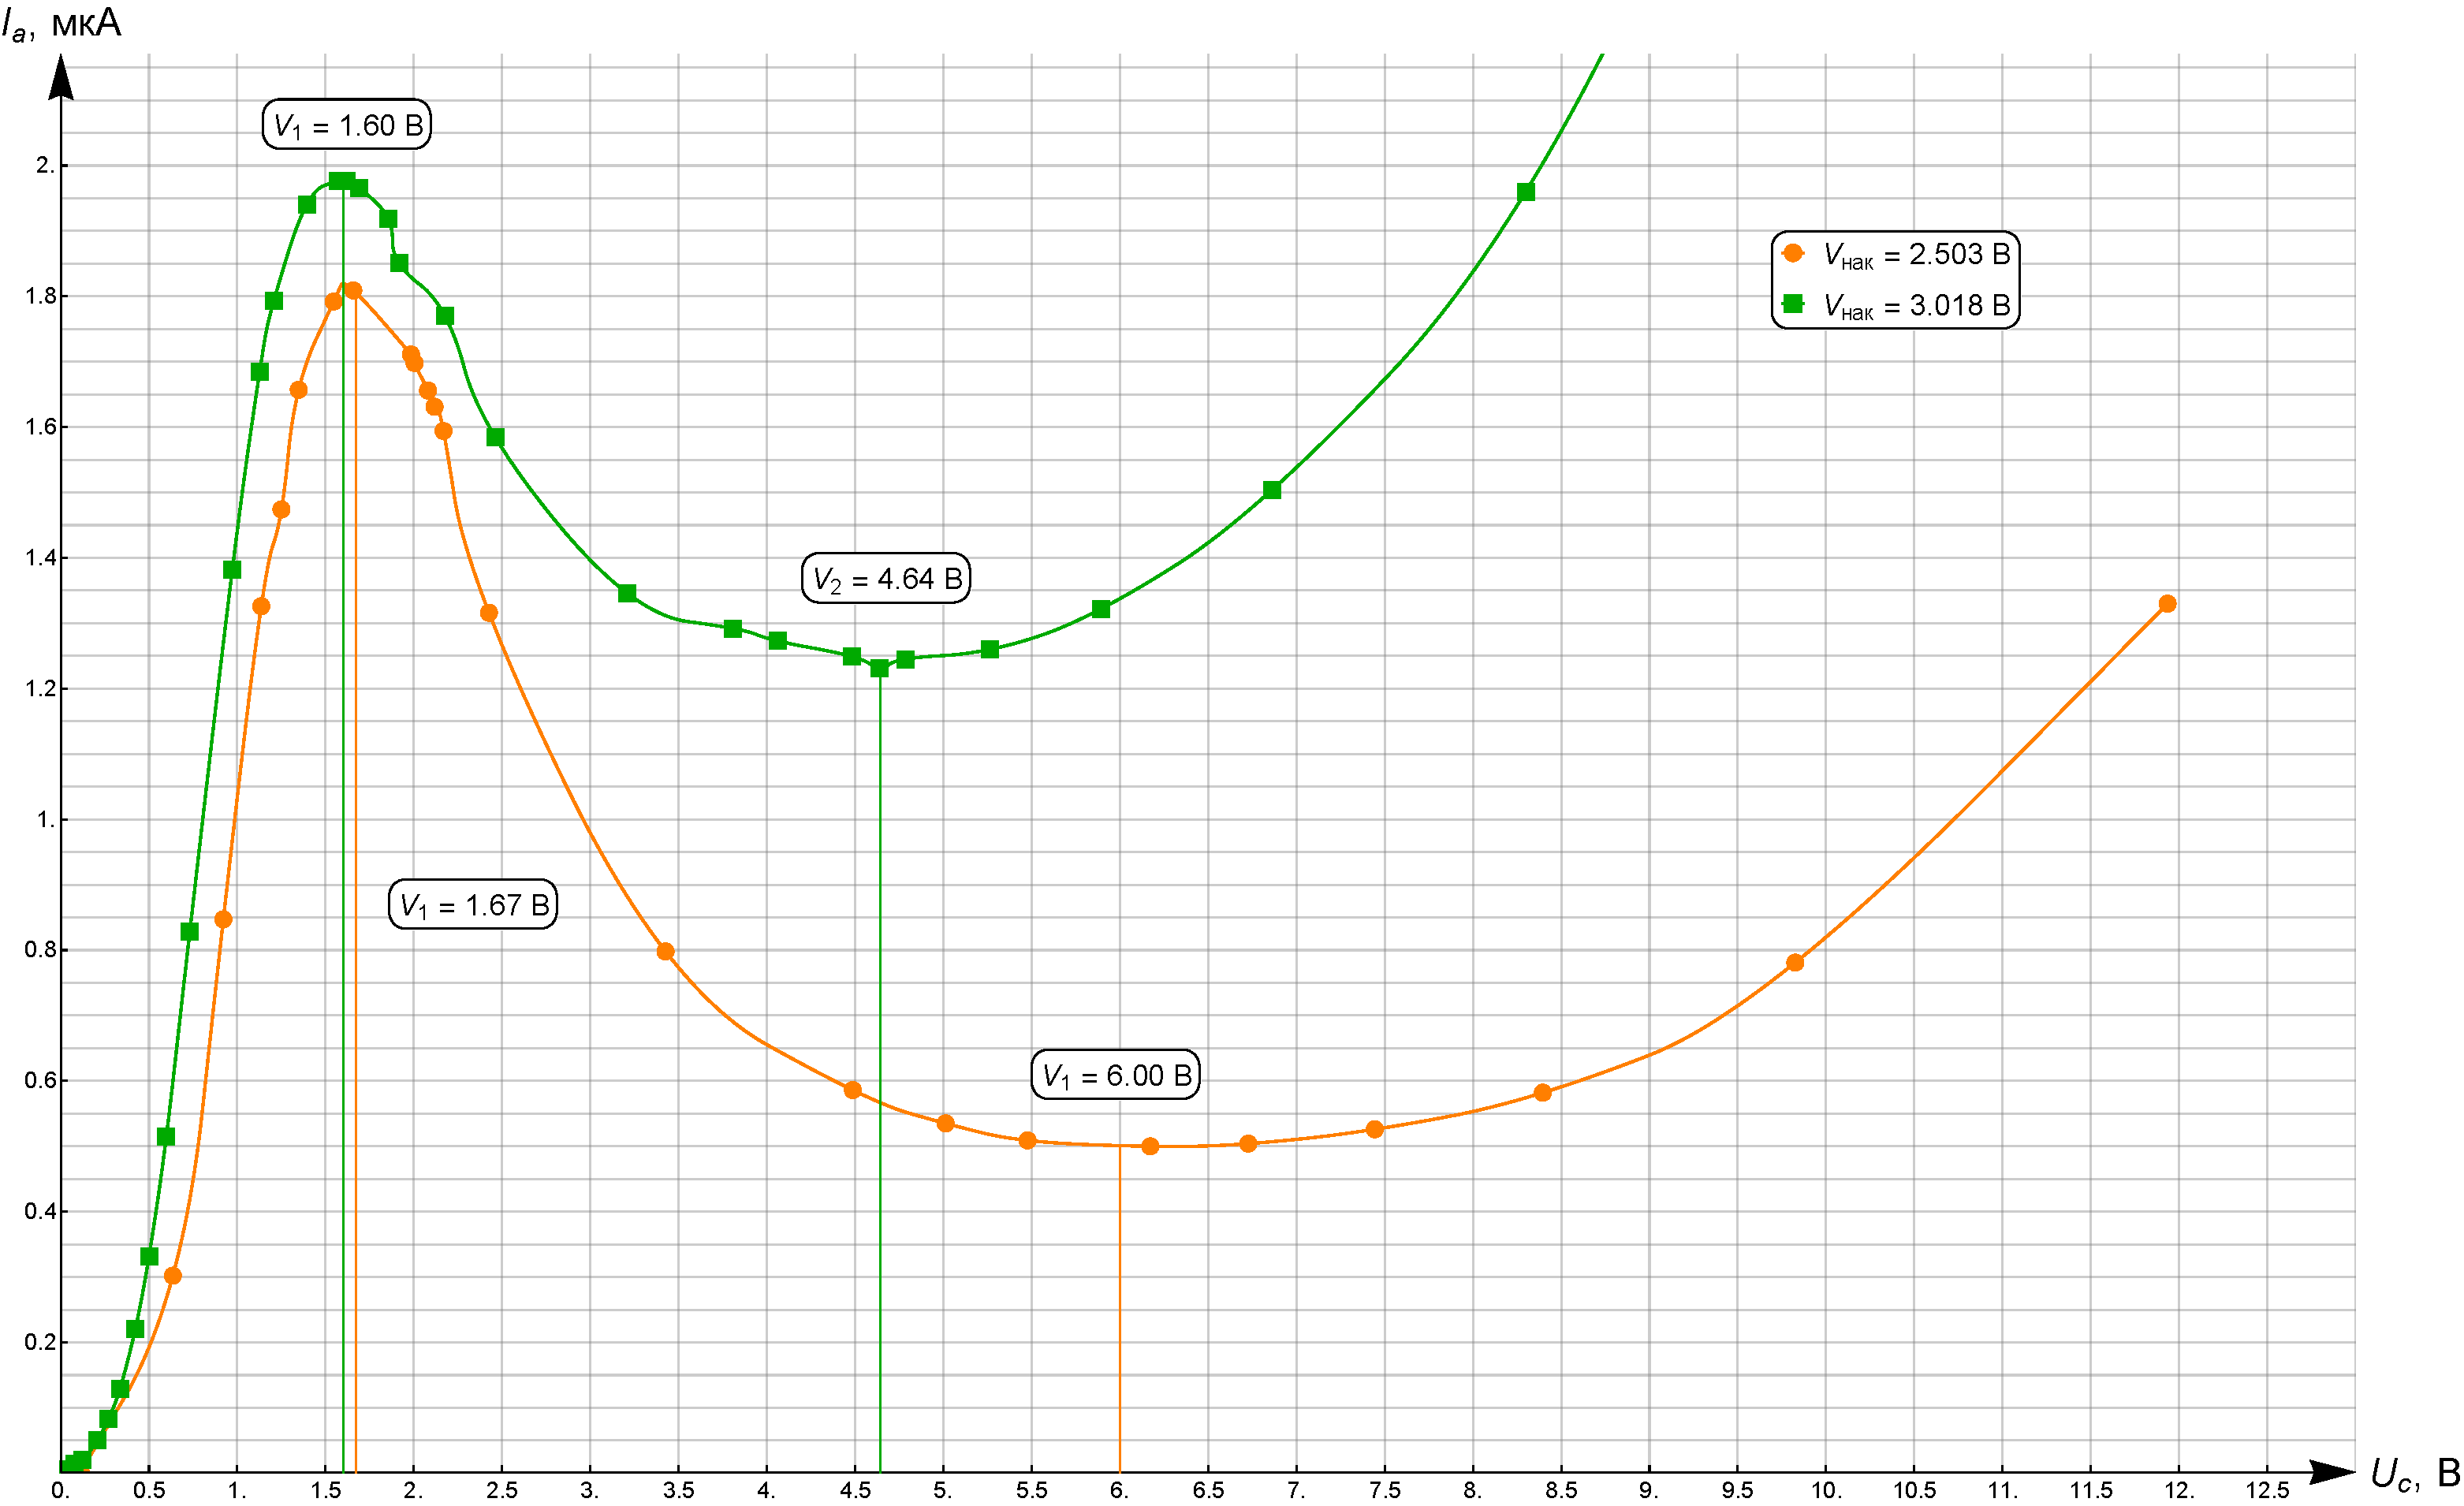
\includegraphics[width=0.8\linewidth]{10} 
    \caption{Зависимость радиуса пятна $z_k$ от положения экрана,
    определяемого пересечение $k$-ого луча и главной оптической оси}
    \label{fig:10}
\end{figure}

Для видимого диапазона оптимальное значение $k = 10\div 12$, при этом
радиус пятна $z_k = (4,5 \pm 1,2)\ \text{мкм}$

С помощью последней программы можно также оценить
количество пятен в предыдущей демонстрации, которые соответствуют
нашей
дифракционной оценке $D$. Получится порядка $16$ зон.

\section{Обсуждение результатов и выводы}
В работе была исследована сферическая аберрация при прохождении света
через собирающую линзу \ffig{fig:4}. Были рассмотрены
параметры, влияющие на величину продольной компоненты сферической
аберрации $X$. При увеличении отношения $F_0/H$ минимальное значение
поперечной компоненты сферической аберрации уменьшается, при
увеличении $F_0/H$ --- увеличивается. При неограниченном увеличении
показателя преломления $n$ $X$ стремится к $0$. По заданному значению
$F_0$ и $1/R_1$ программа определяет величинy $1/R_2$ так, чтобы $X$ было
минимально.

Было проверено правило <<4П>> --- <<плоской поверхностью к плоской
волне плохо>> для плоско-выпуклой линзы. Правило хорошо подтверждается,
при этом величина аберрации в среднем уменьшается в $2$ раза (\textsl{Таблица
\ref{table:1})}.

Рассмотрена сферическая аберрация на паре собирающих линз, плотно
прижатых друг к другу \ffig{fig:5}. При правильном подборе радиусов
линз можно практически убрать сферическую аберрацию.
В работе продольная компонента уменьшилась с $X=0,761$
до $X = 0,026$. Программе задается фокусное расстояние системы
$F_0$ и она подбирает
оптимальные кривизны обеих линз. При этом форма линз, которую можно
восстановить по значениям кривизн поверхностей $1/R_1<0 ,\ 1/R_2>0,
1/R_3<0, 1/R_4<0$ \ffig{fig:3}, подобранным
программой, совпадет с формой, предлагаемой во втором издании книги
(при $F0 = 4,6155$, $H = 2,4949$)
<<\textit{Lens Design Fundamentals}>>, \textit{Rudolf~Kingslake,
R.~Barry Johnson} (иллюстрация с 185 страницы).

\begin{figure}[H]
    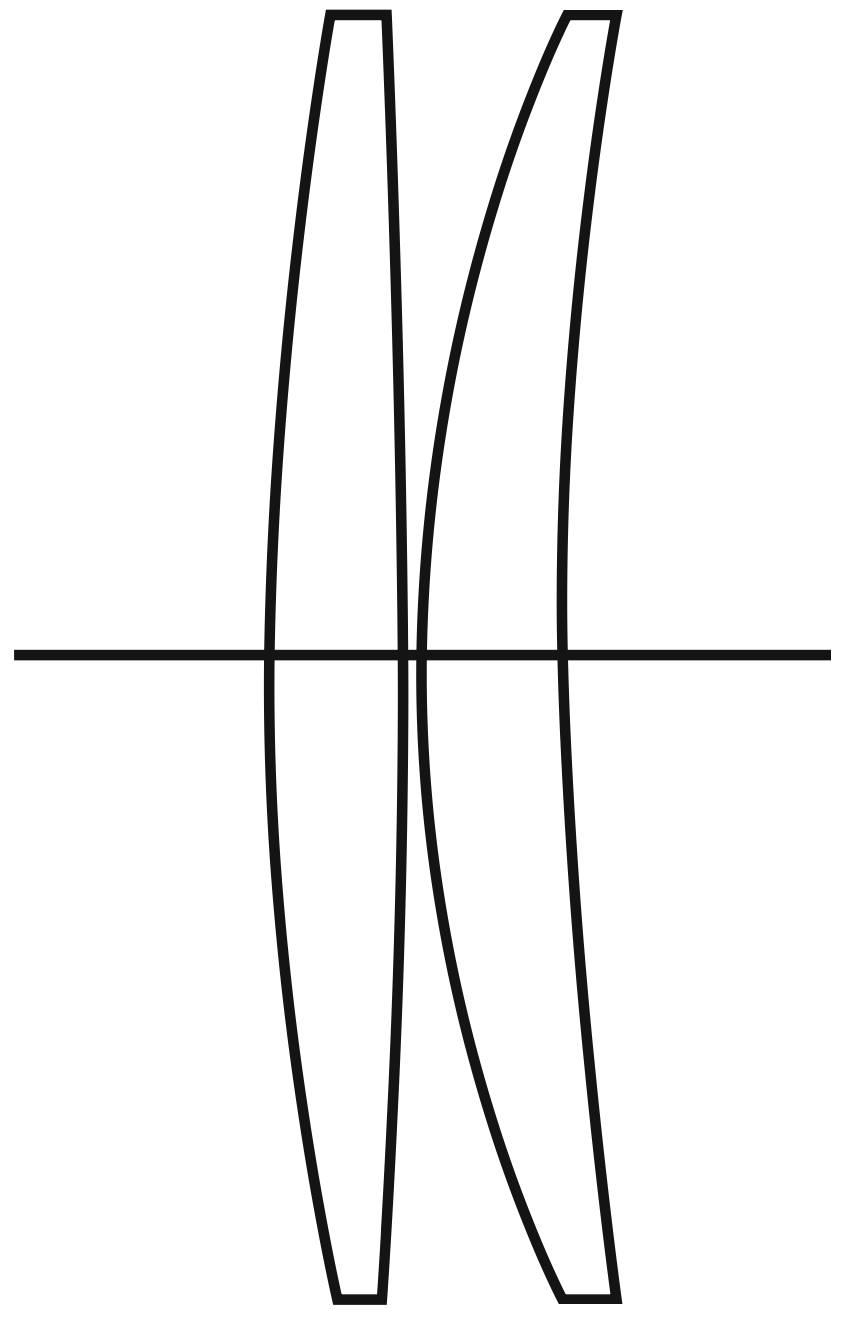
\includegraphics[width=0.2\linewidth]{11} 
    \caption{A two-lins minimum aberration system}
    \label{fig:11}
\end{figure}


На \fig{fig:3} геометрическая оптика предсказывает нам, что экран
нужно ставить в двойной фокус $\text{Э}_2$. Однако при таком
расположении экрана из \fig{fig:9} видно, что максимальная
интенсивность света сосредоточена в очень маленьком кружке, 
размер которого меньше дифракционной оценки $D$.

При последовательном перемещении экрана можно подобрать оптимальное положение радиуса
пятна \ffig{fig:10}. При этом получается, что наибольший вклад в
интенсивность дают всего лишь $12$ зон из $100$. 

\end{document}
